\documentclass[conf]{new-aiaa}
\usepackage[utf8]{inputenc}
\usepackage{booktabs}
\usepackage{caption}
\usepackage{graphicx}
\usepackage{amsmath}
\usepackage[version=4]{mhchem}
\usepackage{siunitx}
\usepackage{longtable,tabularx}
\usepackage{multicol}
\usepackage[inline]{enumitem}
\usepackage[hidelinks]{hyperref}
\usepackage{float}
\usepackage{setspace}

\setlength\LTleft{0pt}
\setlength\parindent{0em}
\setlength\parskip{1em}



% Multifidelity GP/AF
\def\mathbi#1{\textbf{\em #1}}
\newcommand{\DesignVar}{\mathbi{x}}
\newcommand{\DesignMat}{\mathbi{X}}
\newcommand{\DesignSpace}{\mathcal{X}}
\newcommand{\ObjFun}{f}
\newcommand{\MinObjFun}{f^{*}}
\newcommand{\MinDesignVar}{x^{*}}
\newcommand{\LevFid}{l}
\newcommand{\MaxLevFid}{L}
\newcommand{\Dim}{d}
\newcommand{\IterOpt}{i}
\newcommand{\Budget}{B}
\newcommand{\Expectation}{\mathbb{E}}
\newcommand{\NoisyObserv}{y}
\newcommand{\IndNumObs}{n} 
\newcommand{\Dataset}{\mathcal{D}}
\newcommand{\NumObs}{N} 
\newcommand{\MeasureNoise}{\epsilon}
\newcommand{\StandDevNoise}{\sigma_{\epsilon}}
\newcommand{\NorDist}{\mathcal{N}}
\newcommand{\MeanFunGP}{\mu}
\newcommand{\CovFunGP}{\kappa}
\newcommand{\StandDevGP}{\sigma}
\newcommand{\KernelMatrix}{\mathbi{K}} 
\newcommand{\IdMatrix}{\mathbi{I}} 
\newcommand{\StandImprov}{Z}
\newcommand{\StandImprovPar}{\xi}
\newcommand{\ConsFact}{\varrho}
\newcommand{\Discrep}{\delta}
\newcommand{\AF}{U}
\newcommand{\EI}{EI}
\newcommand{\MFEI}{MFEI}
\newcommand{\CompCost}{\lambda}
\newcommand{\CumDistFun}{\Phi}
\newcommand{\ProbDensFun}{\phi}
\newcommand{\Probability}{P}
\newcommand{\PhysicsVec}{\boldsymbol{\psi}}
\newcommand{\Improv}{I}
\newcommand{\RegressParam}{\beta}
\newcommand{\ProcessVar}{\varsigma}
\newcommand{\RegressFun}{\upsilon}
\newcommand{\RoughParam}{\varpi}

\newcommand{\Stage}{z}
%\newcommand{\Expectation}{\mathbb{E}}
%\newcommand{\Stage}{z}
\newcommand{\ExpLoss}{\mathcal{L}}
%\newcommand{\Dataset}{S}
\newcommand{\ExpectedReward}{J}
\newcommand{\StageReward}{r}
\newcommand{\State}{s}
\newcommand{\Control}{c}
\newcommand{\Disturbances}{d}
\newcommand{\SysDyn}{\mathcal{F}}
\newcommand{\Policy}{\pi}
\newcommand{\NorVar}{Z}
\newcommand{\CholDec}{C}
\newcommand{\AuxMat}{H}
\newcommand{\TwoAF}{2AF}
\newcommand{\MCiter}{j}



\documentclass[conf]{new-aiaa}
\usepackage[utf8]{inputenc}
\usepackage{booktabs}
\usepackage{caption}
\usepackage{graphicx}
\usepackage{amsmath}
\usepackage[version=4]{mhchem}
\usepackage{siunitx}
\usepackage{longtable,tabularx}
\usepackage{multicol}
\usepackage[inline]{enumitem}
\usepackage[hidelinks]{hyperref}
\usepackage{float}
\usepackage{setspace}

\setlength\LTleft{0pt}
\setlength\parindent{0em}
\setlength\parskip{1em}


\title{Dynamic Multi-Fidelity Modelling of Low Temperature Proton Exchange Membrane Fuel Cell Power Systems for Clean Aviation}

\author{Joseph Whitaker Schaefer\footnote{Doctoral Student, Brahmal Vasudevan Institute for Sustainable Aviation}}
\author{Francesco Di Fiore \footnote{Research Associate, Brahmal Vasudevan Institute for Sustainable Aviation}}
\author{Billy Wu \footnote{ Reader in Electrochemical Design Engineering, Dyson School for Design Engineering}}
\author{Laura Mainini \footnote{Chair in Aerospace Computational Design, Associate Director, Brahmal Vasudevan Institute for Sustainable Aviation, AFAIAA}}
\affil{Imperial College London}



\begin{document}

\newcommand{\htwo}{\text{H}_2}
\newcommand{\hp}{\text{H}^+}
\newcommand{\electron}{\text{e}^-}
\newcommand{\water}{\text{H}_2\text{O}}
\newcommand{\otwo}{\text{O}_2}
\newcommand{\etal}{\textit{et al}. }
\newcommand{\arcsinh}[1]{\text{arcsinh}\left(#1\right)}

\newcommand{\wt}[1]{\tilde{#1}}
% \newcommand{\bj}{\bm{j}}
% \newcommand{\betah}{\bm{\eta}}
% \newcommand{\bc}{\bm{c}}
\newcommand{\diff}{\text{d}}


\maketitle

\section{Nomenclature}

 {
  \renewcommand\arraystretch{1.0}
  \noindent\begin{longtable*}{@{}l @{\quad=\quad} l@{}}
	  LT-PEM  & Low Temperature Proton Exchange Membrane \\
	  LT-PEMFC  & Low Temperature Proton Exchange Membrane Fuel Cell\\
	  BoP &    Balance of Pant \\
	  TMS & Thermal Management System \\
	  WMS & Water Management System \\
	  MEA & Membrane Electrode Assembly \\
	  GDL & Gas Diffusuion Layer \\
	  ORR & Oxygen Reduction Reaction \\
	  UAV & Unmanned Aerial Vehicle \\
	  eVTOL & Electrical Vertical Take-off and Landing\\
	  $\mathcal{O}(\cdot)$ & Order \\
  \end{longtable*}
 }


\section{Introduction}

\lettrine{I}{mmediate} action is required if we are to limit anthropogenic warming to 2 °C by the year 2100 \cite{environmentEmissionsGapReport2024}.
As of 2021, aviation contributed an estimated 4\% of total warming, but projected growth in demand is expected to increase this to between 6 and 17\% by 2050 \cite{klowerQuantifyingAviationsContribution2021}.
Despite consistent incremental improvements in conventional aeroengine technology, there remain challenges with respect to the emission of carbon dioxide, nitrogen oxides, water, hydrocarbons, carbon monoxide, sulphur oxides, particulates, and other pollutants when relying on the combustion of hydrocarbon fuels.
Consequently, there is interest in developing and adopting alternative energy vectors and power systems to facilitate transition towards clean aviation.
Hydrogen fuel cells (FCs) offer a potential route to clean aviation at scale, by generating electrical energy from hydrogen and oxygen emitting only water as a by-product, thus enabling electric aviation and zero emissions at the point of use.
Low temperature proton exchange membrane (LT-PEM) fuel cells are a mature branch of current hydrogen fuel cell technology. They have been the focus of significant development since the early 2000s for automotive and civil applications due to their reliability and preferable dynamic characteristics relative to high temperature (HT)-PEMFCs, and solid oxide fuel cells (SOFCs).

There is currently a global effort to scale LT-PEMFC systems to meet the power requirements of large transport aircraft \cite{weeksZeroAviaReceivesFAA2025, retallackCommercialAircraftManufacturer2023, NEWBORNNExtGeneration, woodScalabilityHydrogenFuel}.
This follows from a period in which academic institutions \cite{kalloFuelCellSystems2013}, industrial \cite{lapena-reyFirstFuelCellManned2010}, and governmental organisations \cite{noll2004investigation} worked to demonstrate fuel cell powered Unmanned Aerial Vehicles (UAVs) and General Aviation (GA) aircraft.
Despite the considerable knowledge gained from the application of LT-PEMFCs to small aircraft, and the existing wealth of experience in the automotive and civil sectors, there are  design, integration, and operational challenges unique to large aircraft that must be addressed before wider adoption becomes possible.
For example, LT-PEMFC systems are complex and dynamical.
Their multi-scale nature means that small-scale multi-physics effects can govern top level system performance.
LT-PEMFC systems for large aircraft will be subject to extreme safety constraints and conflicting design objectives of minimal mass and maximal power and efficiency are expected to force high current density operation under take-off conditions and simultaneously reduce the ability of the thermal management and water management systems to mitigate against flooding, drying, and steep transient temperature gradients which threaten the ability of the cell to provide the required power at take-off. Careful study of these effects in proposed systems are necessary to ensure safe, efficient, and reliable operation, but is not present in existing preliminary design studies of LT-PEMFC aircraft.
As such there are many open questions that must be addressed to enable design and certification of future large LT-PEMFC aircraft, of which the following will be considered; \begin{enumerate*}
	\item Which, if any, dynamic effects threaten the safe operation of future LT-PEMFC power systems under take-off conditions.
	\item How should LT-PEMFC stack and balance of plant systems be designed and scaled to efficiently power large aircraft.
	\item How do top level integration and architectural decisions impact the optimal LT-PEMFC power system design and vice versa.
\end{enumerate*}

In this context, we propose a modelling and methodological framework to capture dynamic multi-scale and multi-physics phenomena and efficiently explore performance charectaristics of LT-PEMFC systems as they scale to meet intense specific power, mass, and safety requirements.
With this, we aim to address challenges in the design, integration, and operation of LT-PEMFC power systems for large future aircraft.


\section{Background} \label{sec:background}
To design safe, efficient, and reliable LT-PEMFC aircraft, it is necessary to understand the ability of the systems onboard to meet aircraft power requirements.
The complex nature of LT-PEMFC power systems necessitates detailed computational modelling of the cell, stack, and balance of plant to accurately evaluate the system response.
Existing preliminary design studies considering LT-PEMFC powered aircraft investigate design challenges for aircraft of differing scales.
Typically, these rely on low fidelity models calibrated against existing stack designs to quickly explore the design space.
Reliance on low-fidelity models limits the ability of these approaches to consider mass transport, thermal, and hydration effects and therefore investigate stack and system scaling.
To position our work, this section will provide an overview of the existing preliminary design study methodologies in subsection \ref{sec:lit}.
We will then introduce the key physical processes limiting cell performance under the extreme operating in subsection \ref{sec:effects}.
Finally we will provide an overview of cell, stack, and balance of plant operation and design to contextualise the system design problem in subsection \ref{sec:design}.

\subsection{Aircraft Design} \label{sec:lit}
Existing preliminary design studies considering LT-PEMFC aircraft have commonly considered a limited range of physical phenomena affecting system performance.
This is due to the computational cost associated with; \begin{enumerate*} \item high fidelity modelling of LT-PEM cells and systems models \item the large number of model evaluations required to characterise a given design\end{enumerate*}.
This subsection will explore modeling approaches of existing studies to establish common practices and identify knowledge gaps.

Commonly, LT-PEMFC aircraft design studies use semi-empirical, one- or zero-dimensional, steady-state, isothermal  models to evaluate the power performance of a cell \cite{nicolayConceptualDesignOptimization2021b,  abukasimPerformanceFailureAnalysis2022a, ngHydrogenFuelCells2019a, parkRefinedSizingMethod2022, chiaramassaroOptimalDesignHydrogenpowered2024a, schmelcherHydrogenFuelCells2022a, sparanoFutureTechnologicalPotential2023a}.
This approach is viable when considering aircraft with  power requirements on a scale similar to commercially available systems developed for automotive use as it allows for calibration against experimental data from representative systems.
This approach has been used to efficiently investigate conceptual design of novel electric GA aircraft \cite{nicolayConceptualDesignOptimization2021b}, and propose detailed system designs for retrofitting onboard existing commuter aircraft \cite{abukasimPerformanceFailureAnalysis2022a}.
Problems arise when this approach is used to investigate the design of large scale systems.
For example multiple studies considering regional aircraft use low-fidelity semi-empirical models calibrated against data from experiments considering cells with an active are of $\mathcal{O}(10)$ cm$^2$ operating at a steady state, under ideal stoichiometry, with a fuel excess, and in a laboratory setting \cite{chiaramassaroOptimalDesignHydrogenpowered2024a, schmelcherHydrogenFuelCells2022a}, whilst others use unpublished data \cite{sparanoFutureTechnologicalPotential2023a}.
These studies consider cells with an active area of $\mathcal{O}(1000)$ cm$^2$, introducing bias by neglecting the impact of area scaling on cell performance, resulting in an overestimate of system performance.
The limitations imposed by low-fidelity models was recognised by Schr\"oder \etal in a study investigating a regional aircraft concept featuring distributed power and propulsion systems \cite{schroderOptimalDesignProton2024}.
To begin addressing them a one-dimensional multi-phase cell model and detailed balance of plant models were developed and calibrated against existing LT-PEMFC systems.
This allowed investigation into the optimal design of a megawatt scale battery hybridised LT-PEMFC system for regional aircraft with distributed propulsion.
The commitment to validating against existing systems forced the selection of a distributed power system architecture to meet to the required power scales.
This demonstrates the need for detailed modeling of LT-PEMFC systems at scale to enable performance assessment of alternative power system architectures and enable informed concept selection and preliminary design for future large LT-PEMFC aircraft.
\begin{center}
	\begin{table}[H]
		\newcolumntype{Y}{>{\centering\arraybackslash}X}
		\begin{tabularx}{\linewidth}{Y Y Y Y Y Y Y Y Y Y}
			\toprule
			Aircraft Class & Dimension & Isothermal & Dynamic & Multi-Phase & TMS & WMS & Reference                                             \\
			\midrule
			GA             & Quasi-One & Yes        & No      & No          & No  & No  & \cite{nicolayConceptualDesignOptimization2021b}       \\
			Commuter       & Zero      & Yes        & No      & No          & Yes & Yes & \cite{abukasimPerformanceFailureAnalysis2022a}        \\
			eVTOL          & Zero      & Yes        & Semi    & No          & No  & No  & \cite{ngHydrogenFuelCells2019a}                       \\
			eVTOL          & ---       & Yes        & No      & ---         & Yes & Yes & \cite{parkRefinedSizingMethod2022}                    \\
			Multi          & Quasi-one & Yes        & No      & No          & Yes & No  & \cite{chiaramassaroOptimalDesignHydrogenpowered2024a} \\
			Regional       & Zero      & Yes        & No      & No          & Yes & No  & \cite{schmelcherHydrogenFuelCells2022a}               \\
			Regional       & Zero      & Yes        & No      & No          & No  & No  & \cite{sparanoFutureTechnologicalPotential2023a}       \\
			Regional       & One       & Yes        & No      & Yes         & Yes & Yes & \cite{schroderOptimalDesignProton2024}                \\
			\bottomrule
		\end{tabularx}
		\label{tab:studies}
		\medskip
		\caption{A listing of key LT-PEMFC model features from preliminary design studies.}
	\end{table}
\end{center}

\subsection{Dynamic Effects} \label{sec:dyn}
Currently, there is limited consideration for the impact of dynamic effects on the performance of proposed LT-PEMFC systems.
This in spite of the fact that the preferable dynamic response of LT-PEM cells has helped motivate their development and thereby the current maturity and viability for use in aviation.
Dynamic system response has been considered for eVTOL design using a reduced order model to capture LT-PEMFC system transients via a representative circuit \cite{ngHydrogenFuelCells2019a}, however in the context of large aircraft, there are no studies known the authors that consider dynamic effects.
We believe that dynamic effects have the potential to significantly impact the performance of LT-PEMFC systems, particularly under high current density operation.
This may threaten the ability of systems to provide sufficient power at take-off where the highest power demand is traditionally imposed, and the lowest temperature difference is available to the Thermal Management System (TMS) for heat rejection.
This is intensified under  traditional aircraft design objectives such as lightweighting and fuel consumption, which will incentivise smaller stacks, TMS, water management systems (WMS), and higher current densities.
To justify this belief, we will introduce the basic physical processes governing key dynamic processes.

In a LT-PEM cell, there exists opposing needs to hydrate the membrane and avoid flooding pores, which may be controlled by varying the humidification of the reactant flows. Under high humidification, water may condense and flood pores in the electrodes, even at low current densities.
This is exacerbated at the cathode, where the Oxygen Reduction Reaction (ORR) forms water.
The resulting impedance of oxygen transport to the cathode causes in a reduction of the cell voltage due to low local oxygen availability.
Under low humidification there is the potential for membrane drying, which prevents the transport of protons across the membrane, and limits reaction rates at the electrodes.
High temperatures in the electrode result in an increased reactant gas saturation pressure, driving greater evaporation and increasing the mass of water removed.
This can mitigate against flooding or accelerate drying depending on the operating conditions of the cell.
High temperature gradients in the cathode and the adjacent GDL can induce flooding as the saturation pressure of the reactant decreases in a non-linear fashion as the gas cools.
If the saturation decreases below the partial pressure of the water vapour, liquid water condenses.
This typically occurs in the GDL or channels, blocking the transport of reactants and causing losses due to reduced local reactant concentration.
Simultaneous flooding and drying is possible under high temperatures and steep temperature gradients, caused by high current density operation, as water is removed from the membrane and deposited elsewhere.
We believe that the design of the cell, stack, and balance of plant will be influenced by the abiltiy of the TMS and Water Management Systems (WMS) to manage flooding, drying, and temperature gradients at take-off.
To investigate this belief detailed dynamic modeling of the cell, stack, TMS, and WMS is required, including high-fidelity models that capture these effects.

\subsection{Cell, Stack, \& Balance of Plant} \label{sec:design}
To formulate the design problem we aim to investigate using our proposed methodology, we must introduce the design of LT-PEMFC power systems. This section aims to provide a brief overview of these components and outline their influence on system performance.

Hydrogen fuel cells utilise a reaction between oxygen and hydrogen to convert between chemical potential and electrical energy.
At the cathode, gaseous oxygen is reduced to water, and at the anode gaseous hydrogen is oxidised to H$^+$ ions as per the half reactions given in equations \ref{eq:hor} and \ref{eq:orr}.
An ionomer membrane facilitates the transport of protons between cathode and anode via an acidic electrolyte, while porous electrodes facilitate the transport of reactant gasses to the reaction sites.
The electrode pores are infused with catalyst nanoparticles, typically platinum, often supported on carbon particles dispersed throughout the ionomer matrix.
This structure increases the surface area available for reactions to occur, and facilitates the interaction of gaseous fuel, solid catalyst, and dissolved ion, known as three-phase contact.
Together the gas diffusion layer (GDL), electrode, and membrane form the membrane electrode assembly (MEA).
MEA designs are complex, the chemical composition of the membrane, catalyst particle size distribution, GDL microstructure, and other factors of vastly different length scales all impact cell performance.
\begin{align}
	2\htwo             & \rightarrow 4 \hp + 4 \electron \label{eq:hor} \\
	\otwo + 4\electron & \rightarrow 2\water \label{eq:orr}
\end{align}
To increase operating power and voltage, cells are connected in series.
Joining two cells is the bipolar plate, which serve a number of functions.
Beyond facilitating electrical connection between the cathode and anode of adjacent cells, bipolar plates distribute gas across the GDL, remove heat from the system through internal coolant flow, transfer and resist mechanical loads, and provide structural support to the GDL, electrodes, and membrane.
The design of the bipolar plate is therefore tightly coupled with the performance of the balance of plant subsystems.
Larger feed flow and coolant flow channels aid convection reducing pressure losses and easing performance requirements on fluid supply systems.
Simultaneously reducing the area available to conduct charge, thickening the plate which increases Ohmic losses, cell mass, and rigidity.
Smaller channels provide the inverse benefits and limitations.
For any proposed bipolar plate design solution there is a multi-objective trade off between gas supply, structural, mass, water, thermal, and electrical objectives.
Thickness and material requirements of bipolar plates mean they constitute a significant proportion of the stack mass.
For these reasons, bipolar plate design is a common area of study in fuel cell design optimisation, and a range of strategies have been applied to improve their design \cite{liReviewBipolarPlates2005}.

The balance of plant comprises all systems required to monitor and control the operation of a fuel cell stack. This may include, but is not limited to; \begin{enumerate*}
	\item Thermal management
	\item Water management
	\item Fuel Supply
	\item Air supply
	\item Power Distribution
\end{enumerate*}. It comprises a significant portion of the system mass and imposes a significant parasitic loss. Preliminary design studies that separate stack and BoP mass commonly propose systems where the two are comparable, or the BoP is multiples of that of the stack. \cite{schroderOptimalDesignProton2024, parkRefinedSizingMethod2022, schmelcherHydrogenFuelCells2022a}.
There is currently significant uncertainty in the relative contributions of BoP systems to total mass;
The distributed power architecture concept proposed by Schr\"oder \etal massed the TMS at 7.4\% of the system mass and the humidifiers at 16.1\% of system mass \cite{schroderOptimalDesignProton2024}.
Conversely, the more conventional two-nacelle architecture proposed by Schmelcher massed the TMS at 44\%, with no consideration of WMS mass \cite{schmelcherHydrogenFuelCells2022a}.
The level of detail in the modeling approaches of both works are sugnificant, as are their choices of power system architecture.
The discrepancy in sizing of the BoP systems of reinforces the previous conclusions on the importance of detailed modeling when investigating optimal aircraft and power system design.

\section{Methodology} \label{sec:method}

To address the identified gaps and support the goal of designing efficient, reliable, and safe LT-PEMFC systems for aircraft, the authors are developing:

\begin{enumerate}
	\item Dynamic multi-scale and multi-physics LT-PEM cell models.
	\item Parametric stack, TMS, WMS, fuel supply, and air supply models.
	\item Advanced physics-aware machine learning LT-PEMFC stack surrogates.
	\item A computational framework for dynamic fuel cell system modelling.
	\item Advanced computational methods to efficiently explore optimal system design.
\end{enumerate}

Together these actions aim to help the community understand the impact of LT-PEMFC power system transients at take-off, and begin tackling challenges surrounding the integration of these systems on board future large transport aircraft.

\subsection{Cell Modelling}

The physical processes necessary for the operation of LT-PEMFCs occur across a wide range of length scales. The catalysed ORR at a three-phase boundary and transport of water across the ionomer are governed by molecular level physics. Simultaneously the convective transport of reactants occurs first over the cell width, and second, through pores of diameter smaller than the mean free path of the gas molecules. These multi-scale mass, momentum, species, charge, and energy transfers are tightly coupled, resolving them fully is infeasible with current computational capability.

\noindent
\begin{minipage}[t]{\linewidth}
	\begin{align}
		\frac{\partial(\epsilon C_k)}{\partial t} + \nabla (\vec{u} + C_k)                                        & = \nabla(D_k^{\text{eff}} \nabla C_k) + S_k               & \frac{\partial(\rho c_p)_mT}{\partial t} + \nabla(\rho c_p \vec{u} T) & = \nabla(k_{\text{eff}} \nabla T) + S_T \tag{3a, 3b} \\
		\frac{1}{\frac{\partial( \epsilon \rho \vec{u})}{\partial t}  + \frac{1}{\nabla (\rho \vec{u} \vec{u})} } & = -\nabla p + \nabla \tau + S_u                           &
		\frac{\partial(\epsilon \rho)}{\partial t} + \nabla(\rho \vec{u})                                         & = S_m                                        \tag{4a, 4b}                                                                                                                                \\
		\nabla(\kappa^{\text{eff}} \nabla \Phi_e)                                                                 & = -S_\Phi                                                 &
		\nabla(\sigma^{\text{eff}}\nabla\Phi_s)                                                                   & = S_\Phi \tag{5a, 5b}
	\end{align}
\end{minipage}%
\hfill\vspace{1em}
\begin{minipage}[t]{\linewidth}
	\begin{center}
		\captionof{table}{Source terms for the single-phase fuel cell model presented by [wang]}
		\newcolumntype{V}{>{\hsize=.4\hsize}>{\raggedright\arraybackslash}X}
		\newcolumntype{Y}{>{\centering\arraybackslash}X}
		\newcolumntype{Z}{>{\hsize=.5\hsize}>{\centering\arraybackslash}X}
		\begin{tabularx}{\linewidth}{V Z Y Z}
			\toprule
			                & Gas Diffusion Layer             & Catalyst Layer                                                                      & Membrane                                  \\
			\midrule
			Mass (4b)       &                                 & $S_m = \sum_k M_k S_k + M_{\water} \nabla (D_{w,m} \nabla C_{\water})$              &                                           \\
			Momentum (4a)   & $S_u = -\vec{u}(\frac{\mu}{K})$ & $S_u = -\vec{u}(\frac{\mu}{K})$                                                     & $\vec{u} = 0$                             \\
			Species (3a)    &                                 & $S_k = -\nabla\left( \frac{n_d}{F} i_e\right) - \left( \frac{s_k j}{nF}\right)$     & $-\nabla\left( \frac{n_d}{F} i_e\right)$  \\
			Charge (5a, 5b) &                                 & $S_\Phi = j$                                                                        &                                           \\
			Energy (3b)     &                                 & $S_T = j\left( \eta + T \frac{dU_0}{dT}\right) + \frac{i_e^2}{\kappa^{\text{eff}}}$ & $S_T = \frac{i_e^2}{\kappa^{\text{eff}}}$ \\
			\bottomrule
		\end{tabularx}
	\end{center}
\end{minipage}

Commonly, when investigating cell and stack polarisation, assumptions of continuity allow diffusive processes to be modelled without resolving pore scale effects. This allows for the derivation of Partial Differential Equations (PDEs) commonly solved via finite element methods and finite volume methods. Often, a single set of equations is applied over the full domain of a cell, with the response of different subdomains governed by their source terms. One such set of PDEs, presented by [wang], is given in table 2. A wide range of PDEs of differing fidelities are presented throughout literature, trading computational cost against physics complexity.

Open-source fuel cell models are of interest in this work as they provide an efficient approach to incorporating multiple model fidelities. A non-exhaustive list of open-source models are presented in table [].

\begin{center}
	\begin{table}
		\caption{Do This}
		\newcolumntype{Y}{>{\centering\arraybackslash}X}
		\newcolumntype{Z}{>{\hsize=.65\hsize}>{\centering\arraybackslash}X}
		\newcolumntype{V}{>{\hsize=.4\hsize}>{\centering\arraybackslash}X}
		\begin{tabularx}{\linewidth}{V Y Z Z Z Z}
			\toprule
			Authors     & Vetter \& Schumacher & Secanell \etal & Zhang \etal & Kone \etal & Gass \etal \\
			\midrule
			Dimension   & One                  & Up to three    & Three       & Three      & One        \\
			Isothermal  &                                                                               \\
			Water Phase & Multi                & Multi          & Multi       & Single     & Multi      \\
			\bottomrule
		\end{tabularx}
		\label{tab:opensource}
	\end{table}
\end{center}

\subsection{Surrogate Modelling}

[Autoregressive Multi-fidelity GPs]

[Active learning, and Bayesian Optimisation]

[Non-myopic Bayesian optimisation]

[Proposed Fuel Cell Stack Surrogate]

\subsection{Dynamic Fuel Cell System Model}

A computational framework for dynamic fuel cell system modelling has been developed by the authors to allow modular development and simple composition of fuel cell system component models. This has been accompanied by implementation of the following sub-models from the work of Pukrushpan et al \cite{pukrushpan_control_2004}.
\begin{multicols}{2}
	\begin{itemize}
		\item Electric Motor
		\item Compressor
		\item Manifold
		\item Humidifer
		\item Cathode
		\item Anode
		\item Membrane Hydration
		\item Stack Voltage
	\end{itemize}
\end{multicols}
\vspace{-1em}
The resulting LT-PEMFC power system model has been validated against the work of Pukrushpan et al, as demonstrated in Figures \ref{} and \ref{}.

\noindent
\begin{minipage}[t]{\linewidth}
	\begin{center}
		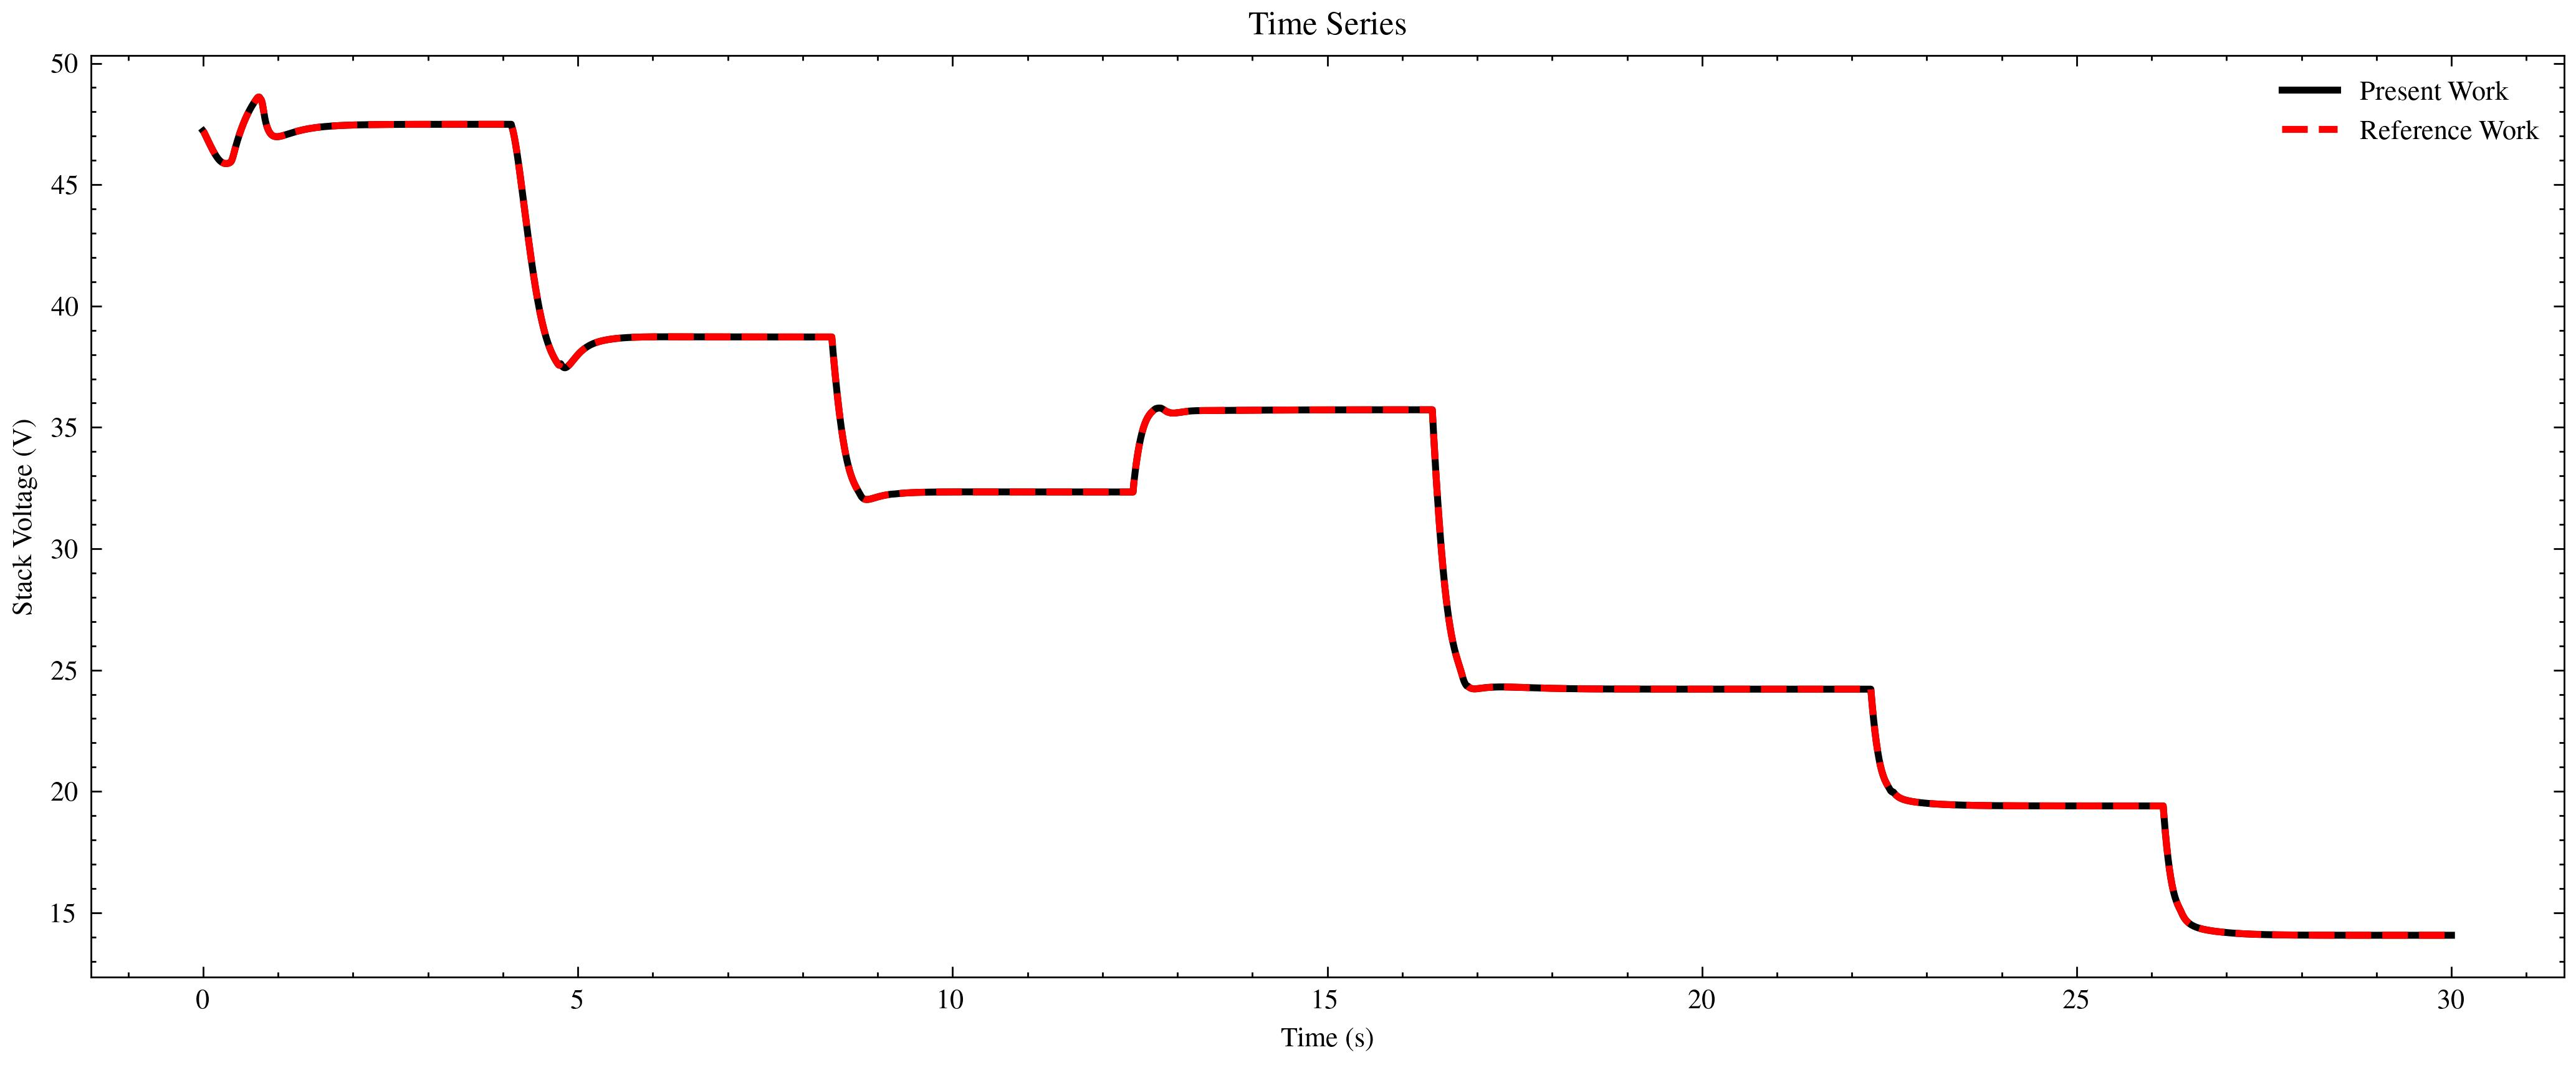
\includegraphics[height=18em]{figures/voltage_ts.jpg}
		\captionof{figure}{Some caption}
	\end{center}
\end{minipage}%
\hfill\vspace{1em}
\begin{minipage}[t]{\linewidth}
	\begin{center}
		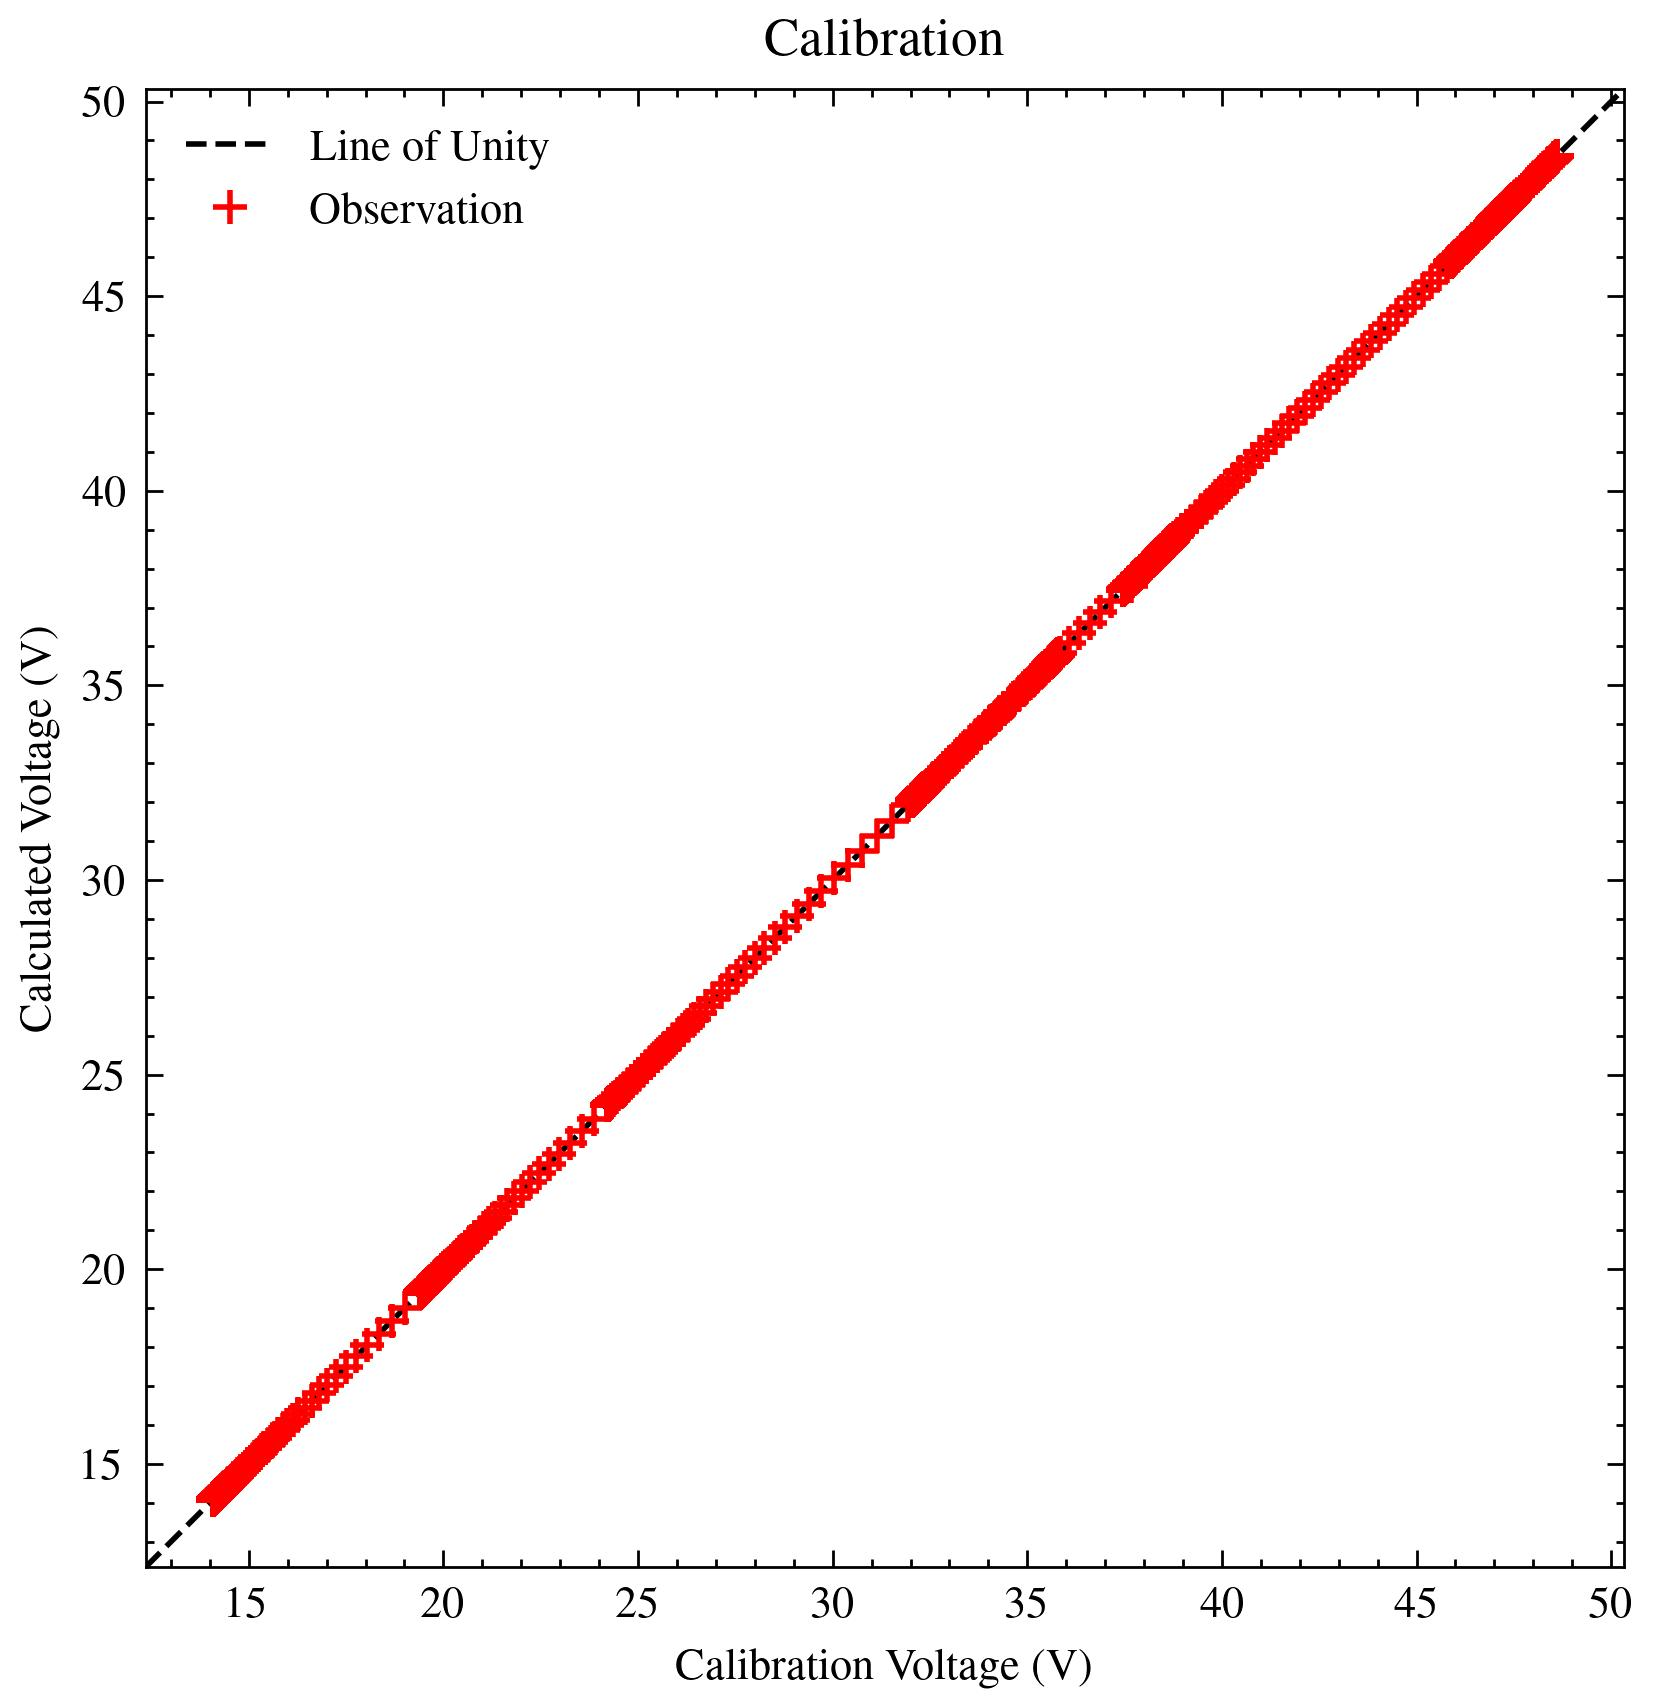
\includegraphics[height=18em]{figures/voltage_cal.jpg}
		\captionof{figure}{Some caption}
	\end{center}
\end{minipage}

Future work is planned to implement sub-models for future LT-PEMFC aircraft systems. This will include water management, thermal management, air supply, and fuel supply systems. The response of a given stack design evaluated using the stack surrogate model described in section []. The system dynamic response is evaluated using an implicit adaptive Runge-Kutta integrator. An XDSM diagram of the proposed study is presented in figure \ref{fig:xdsm}.

\begin{center}
	\begin{figure}
		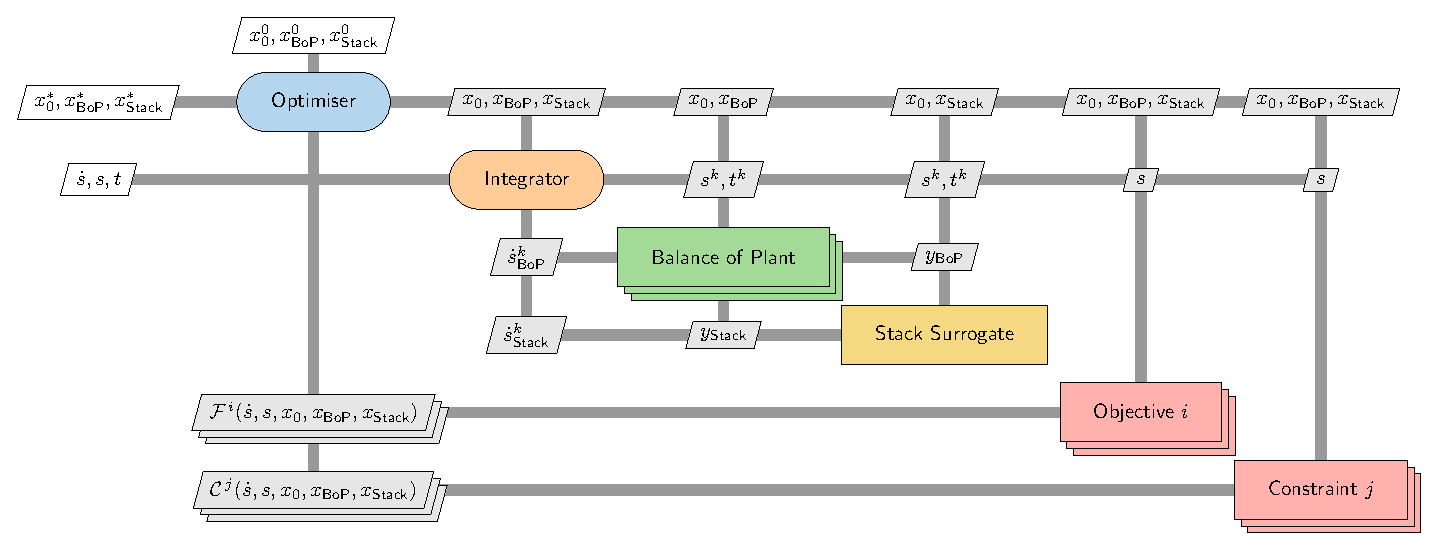
\includegraphics[width=\linewidth]{figures/xdsm.pdf}
		\caption{XDSM Diagram of the proposed fuel cell system model}
		\label{fig:xdsm}
	\end{figure}
\end{center}

\subsection{Design Optimisation}


\section{Preliminary Results}
The dynamic system modelling framework has been implemented and validated.
An automotive fuel cell system presented by Pukrushpan \etal \cite{pukrushpanControlFuelCell2004a} was chosen as a validation case due to the availability the source code to the authors and the simple, well documented component models. Following the implementation of said component models, the response of the system to a prescribed stack current profile was evaluated, and compared to the response of the original models. The time-series output of the stack voltage is given in Figure \ref{fig:ts} and a calibration plot is given in Figure \ref{fig:cal}.
\medskip
\noindent
\begin{minipage}[t]{\linewidth}
	\begin{center}
		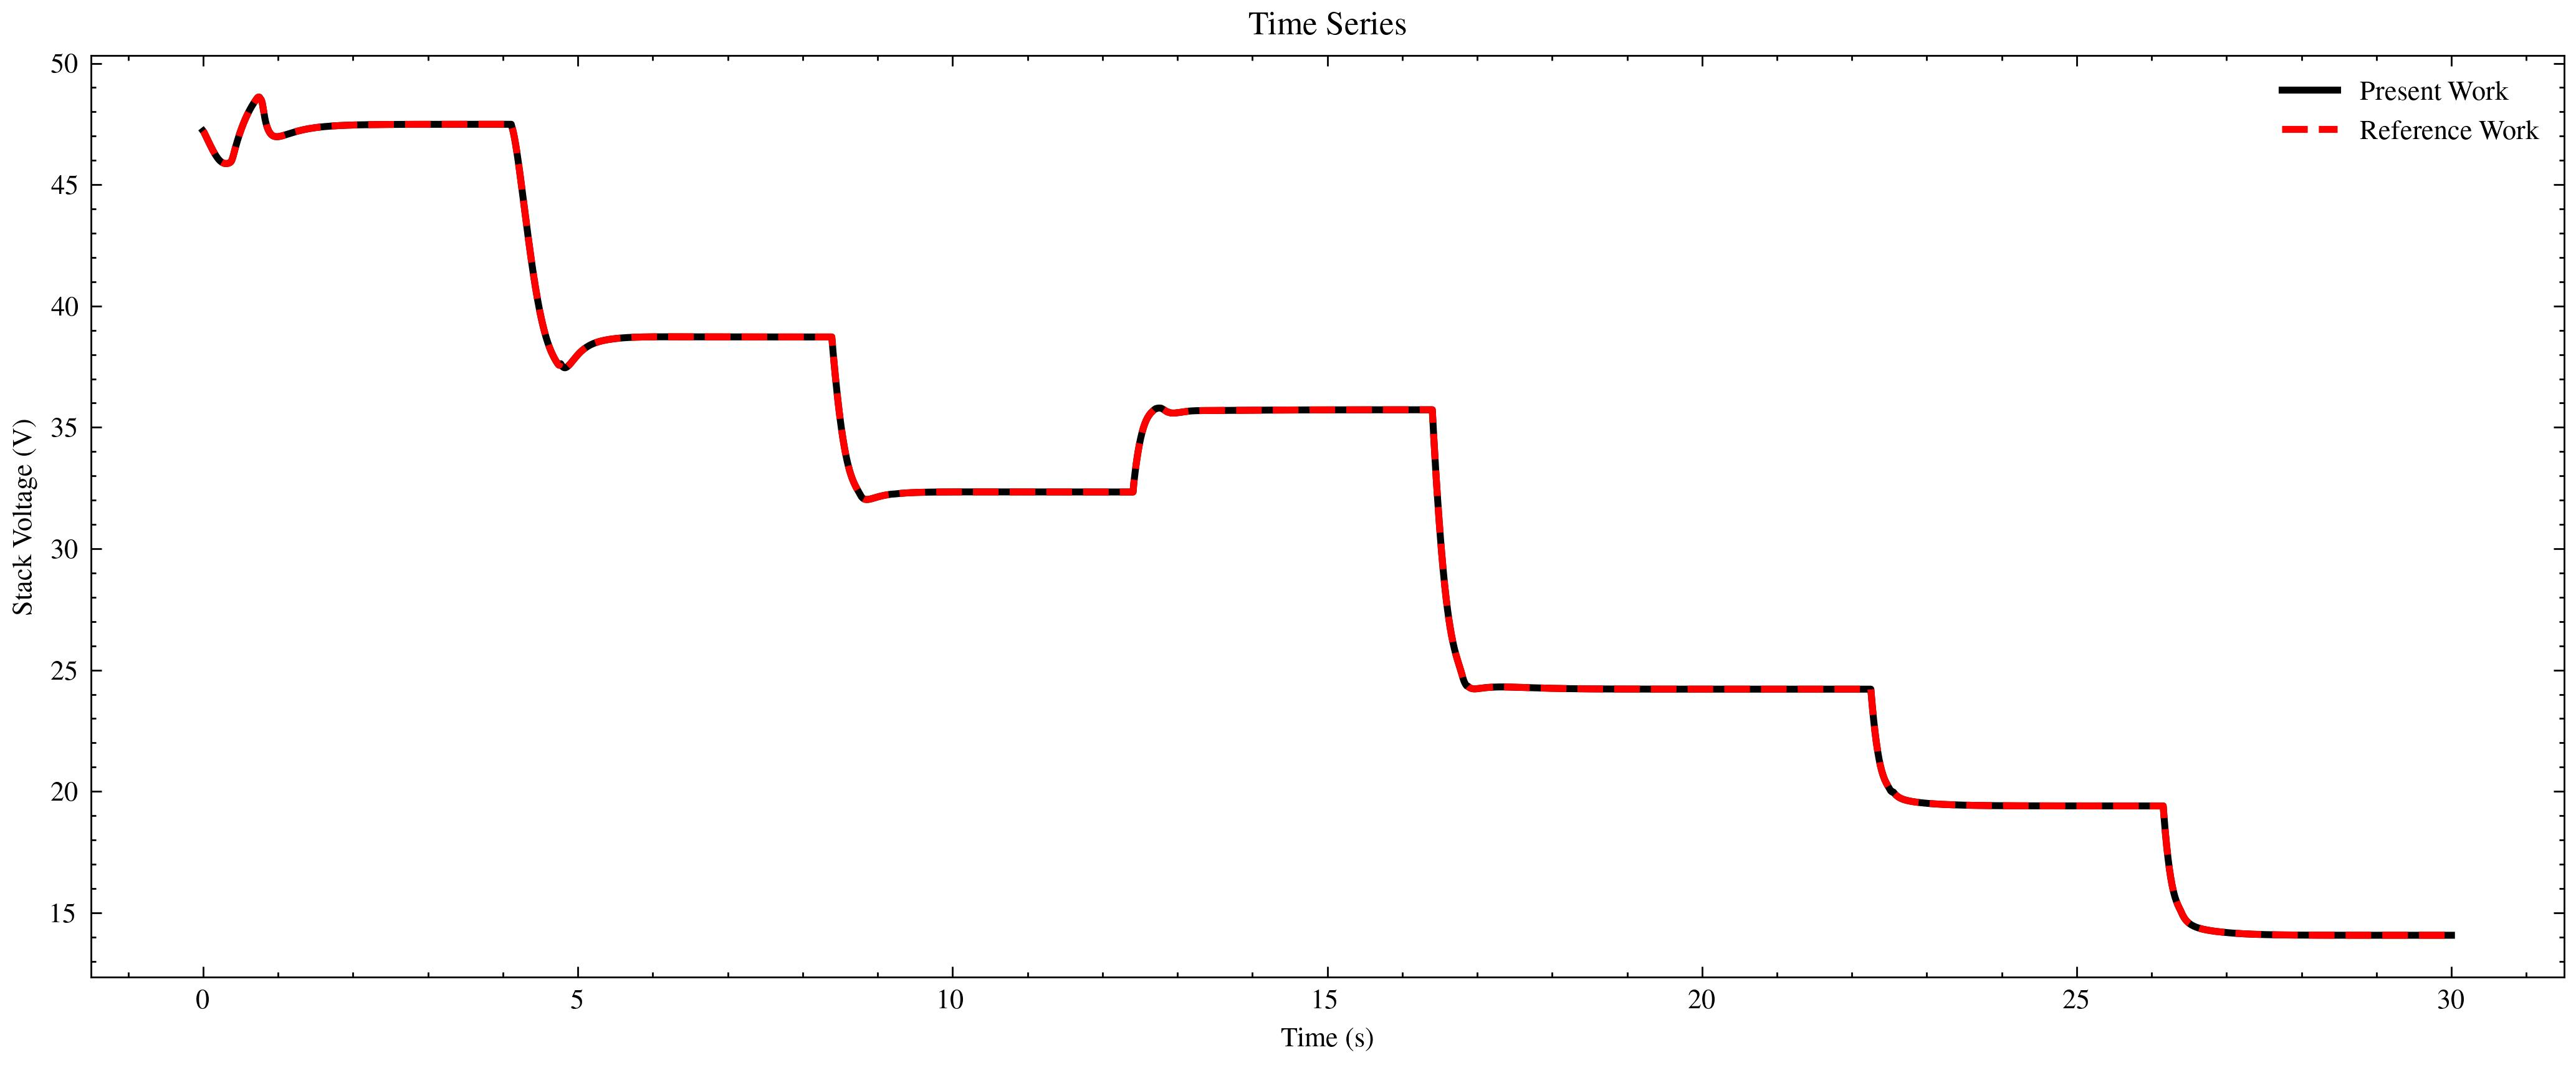
\includegraphics[height=18em]{figures/voltage_ts.jpg}
		\captionof{figure}{Some caption}
		\label{fig:ts}
	\end{center}
\end{minipage}%
\hfill\vspace{1em}
\begin{minipage}[t]{\linewidth}
	\begin{center}
		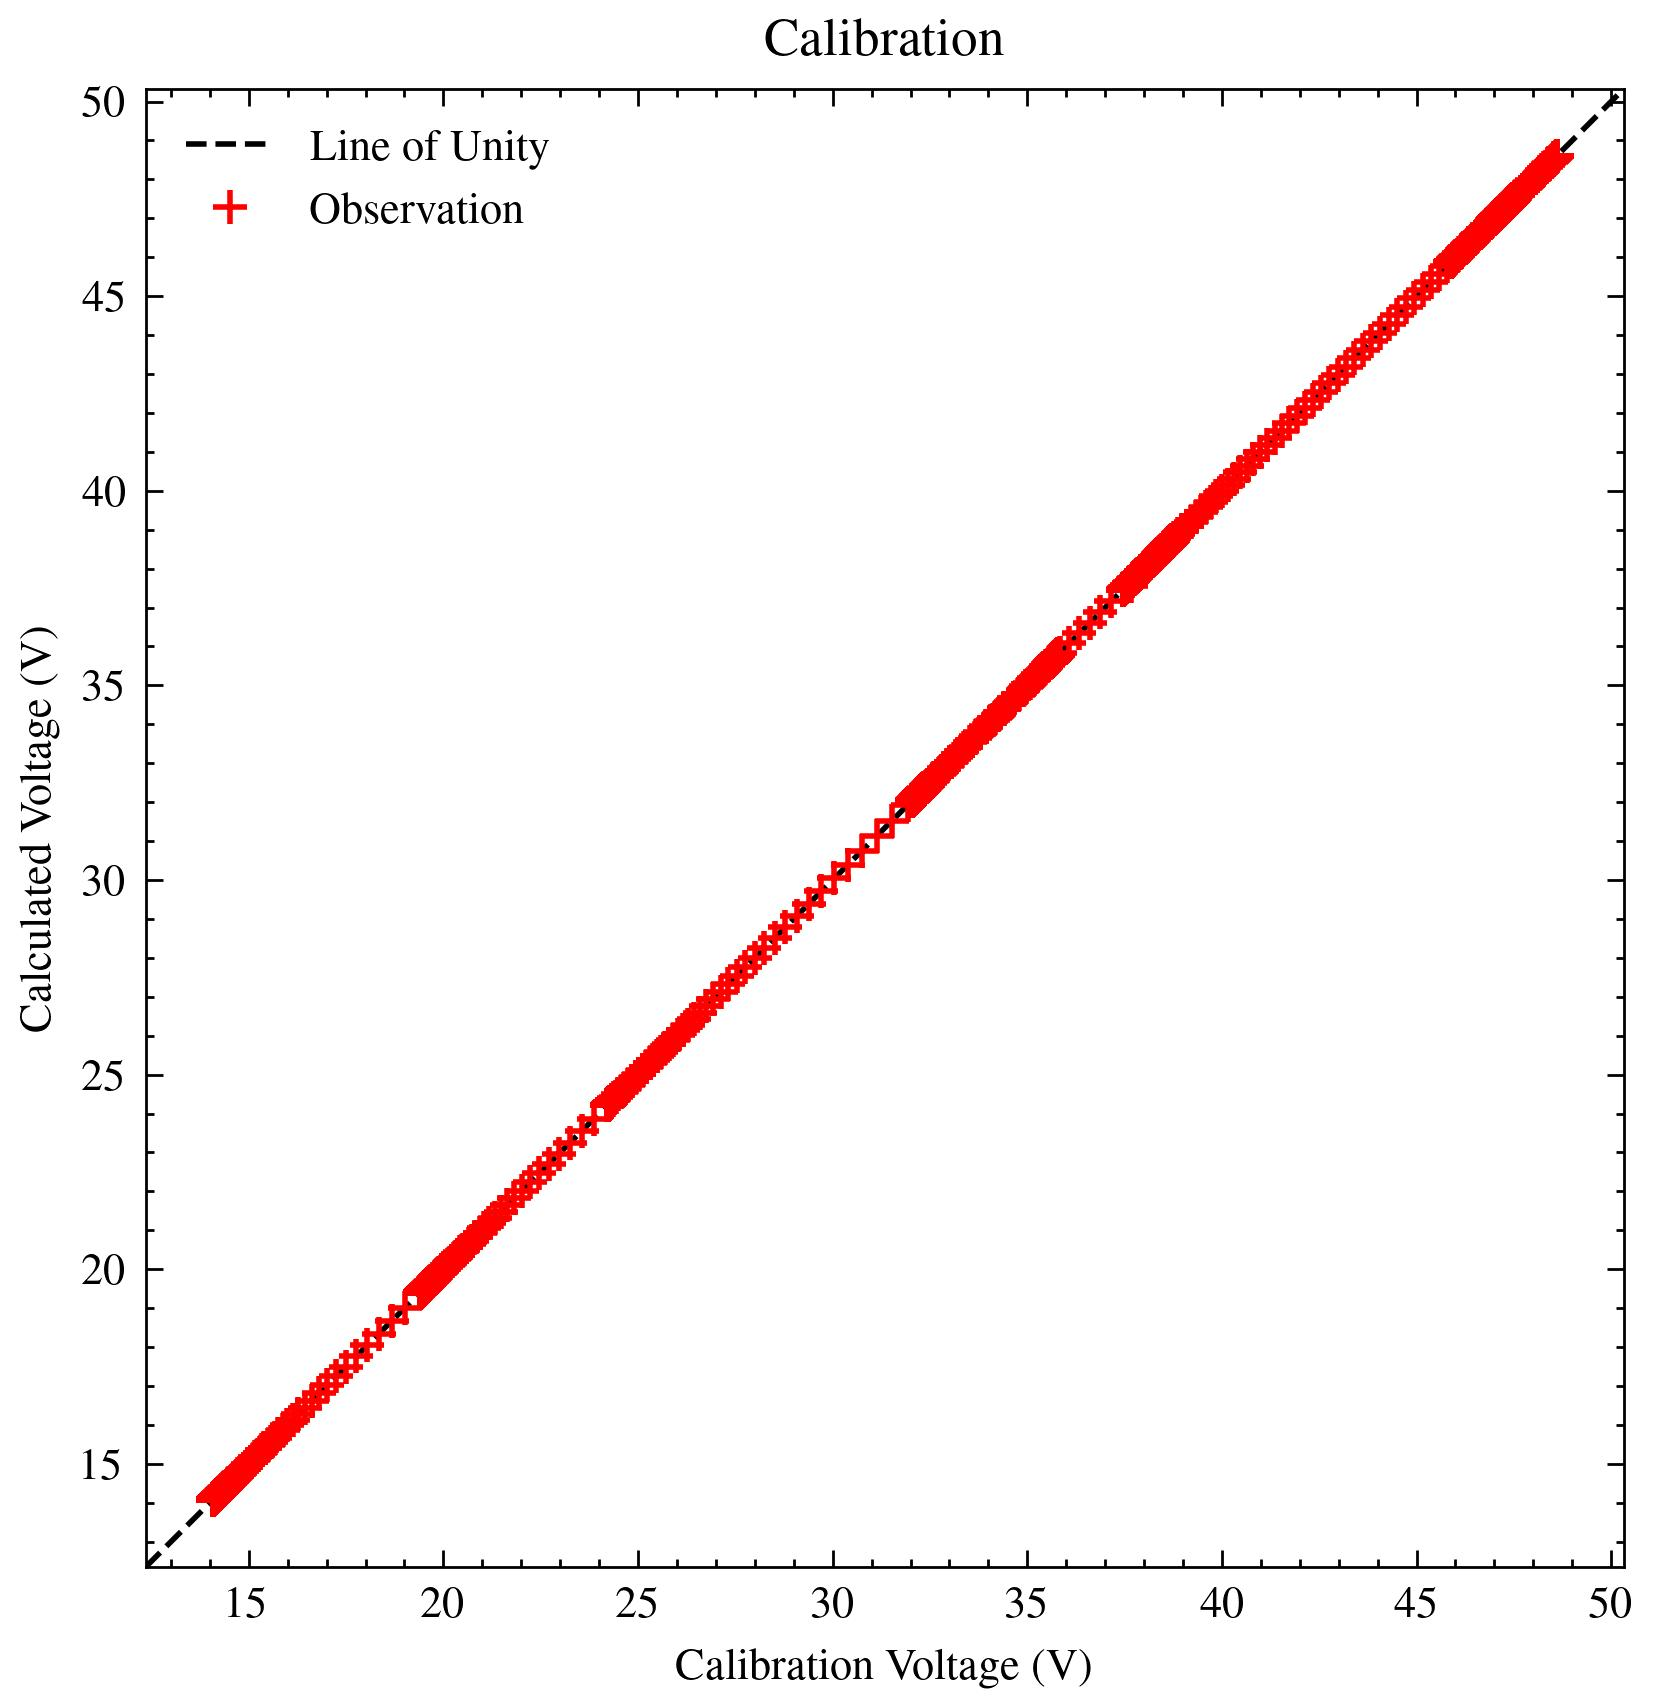
\includegraphics[height=18em]{figures/voltage_cal.jpg}
		\captionof{figure}{Some caption}
		\label{fig:cal}
	\end{center}
\end{minipage}


\bibliography{references, standalone}

\end{document}
